\documentclass[11pt, a4paper]{article}
%\usepackage{proj1}
\usepackage{natbib}
\usepackage{fancyhdr}  
\usepackage{subcaption}
\usepackage{caption}
\usepackage{graphicx}
\linespread{1.25} 
\setlength{\parindent}{0cm}
\graphicspath{{Images/}}
\usepackage{hyperref}
\usepackage{amsmath}
\usepackage{amsfonts}
\usepackage{amssymb}
\usepackage{amsthm}
\usepackage{mathtools}
\usepackage{commath}
\usepackage{bbm}
%\usepackage[sc,osf]{mathpazo}
\usepackage{subcaption}
\usepackage[a4paper, top=1in, left=1.0in, right=1.0in, bottom=1in, includehead, includefoot]{geometry} %Usually have top as 1in

\usepackage{listings}
\usepackage{color} %red, green, blue, yellow, cyan, magenta, black, white
\definecolor{mygreen}{RGB}{28,172,0} % color values Red, Green, Blue
\definecolor{mylilas}{RGB}{170,55,241}


\hypersetup{colorlinks,linkcolor={black},citecolor={blue},urlcolor={black}}
\usepackage{color}
\urlstyle{same}

\newcommand{\Sta}{\rho}
\newcommand{\Stav}{\mathbf{v}}
\newcommand{\Adja}{{p}_Q}
\newcommand{\Adjb}{q}
\newcommand{\Adjc}{p_{\partial Q}}
\newcommand{\Con}{{f}}
\newcommand{\nor}{\mathbf{n}}

\theoremstyle{definition}
\newtheorem{definition}{Definition}[section]


\pagenumbering{gobble}
\begin{document}

\lstset{language=Matlab,%
	%basicstyle=\color{red},
	breaklines=true,%
	morekeywords={matlab2tikz},
	keywordstyle=\color{blue},%
	morekeywords=[2]{1}, keywordstyle=[2]{\color{black}},
	identifierstyle=\color{black},%
	stringstyle=\color{mylilas},
	commentstyle=\color{mygreen},%
	showstringspaces=false,%without this there will be a symbol in the places where there is a space
	numbers=left,%
	numberstyle={\tiny \color{black}},% size of the numbers
	numbersep=9pt, % this defines how far the numbers are from the text
	emph=[1]{for,end,break},emphstyle=[1]\color{blue}, %some words to emphasise
	%emph=[2]{word1,word2}, emphstyle=[2]{style},    
    basicstyle=\footnotesize\ttfamily,
}

\section*{Boundary Observation and Non-Constant Flux Boundary conditions}
This set of notes is concerned with deriving non-zero (non-)constant flux boundary conditions, which are different for different parts of the boundary. 
Furthermore, the target distribution of particles $\hat \Sta$ is prescribed on parts of the boundary only, instead of on all of $\Omega$. Different parts of the boundary have different target distributions of particles.\\
+++ Boundary control correct here, since we don't directly apply the control on the boundary??+++


\begin{figure}[h]
	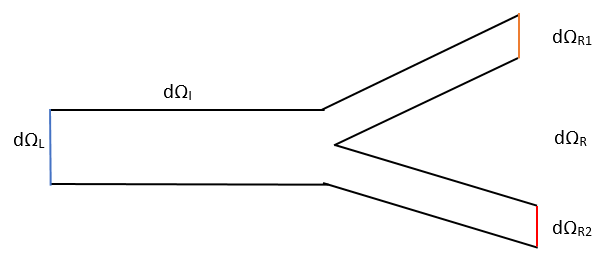
\includegraphics[scale=0.8]{bound.png}
	\caption{Boundary}
    \label{Boundary1}
\end{figure}
The domain with the different parts of the boundary that are considered can be seen in Figure \ref{Boundary1}.

\section{Distributed Observation and Constant Flux Boundary Conditions}
The problem of interest is of the form:
\begin{align*}
&\min_{\Sta, \Con} \quad \frac{1}{2}|| \Sta -\hat \Sta||^2_{L_2(Q)} + \frac{\beta}{2}|| \Con||^2_{L_2(Q)}\\
\text{subject to:}\\
&\partial_t \rho = \nabla^2 \rho - \nabla \cdot (\rho \mathbf{w}_{Flow}) +\nabla \cdot (\rho \nabla V_{ext}) + \nabla \cdot \int_\Omega \rho(r) \rho(r') \nabla V_2(|r-r'|) dr' + \Con \quad  \quad\text{in} \quad Q,\notag\\
& \rho = \rho_0 \quad \text{at} \quad t=0 \notag\\
& - \mathbf{j} \cdot \nor = \mathbbm{1}_{\partial \Omega_L} C_L +\mathbbm{1}_{\partial \Omega_R} C_R +\mathbbm{1}_{\partial \Omega_I} 0,  \quad \text{on} \quad \partial Q, 
\end{align*}
where $C_L$, $C_R$ are constants and $\mathbbm{1}$ is the indicator function of the set (the parts of the boundary) of interest.
Furthermore, $\mathbf{j}$ satisfies:
\begin{align*}
\mathbf{j}=\nabla \rho - (\rho \mathbf{w}_{Flow}) +(\rho \nabla V_{ext}) +  \int_\Omega \rho(r) \rho(r') \nabla V_2(|r-r'|) dr'.
\end{align*}
\subsection*{The Lagrangian}
The Lagrangian is of the form:
\begin{align*}
\mathcal{L}(\Sta,\Con,\Adja,\Adjc ) &= \int_0^T \int_\Omega \frac{1}{2}(\Sta - \hat \Sta)^2 dr dt + \frac{\beta}{2}\int_0^T \int_\Omega \Con^2 drdt \\
&+ \int_0^T \int_\Omega \bigg( \partial_t \rho - \nabla^2 \rho + \nabla \cdot (\rho \mathbf{w}_{Flow}) -\nabla \cdot (\rho \nabla V_{ext}) + \nabla \cdot \int_\Omega \rho(r) \rho(r') \nabla V_2(|r-r'|) \bigg) \Adja dr dt\\
&+ \int_0^T \int_{\partial \Omega} \bigg( \bigg( -\nabla \rho+ (\rho \mathbf{w}_{Flow}) -(\rho \nabla V_{ext}) -  \int_\Omega \rho(r) \rho(r') \nabla V_2(|r-r'|) dr' \bigg)\cdot \nor\\
& -\mathbbm{1}_{\partial \Omega_L} C_L -\mathbbm{1}_{\partial \Omega_R} C_R -\mathbbm{1}_{\partial \Omega_I} 0 \bigg) \Adjc dr dt.
\end{align*}

\subsection*{The Adjoint Equation}
The derivative of $\mathcal{L}$ with respect to $\rho$ is, as taken from the extended project:
\begin{align*}
&\mathcal{L}_\rho (\rho,\mathbf{w},p_\Omega,p_{\partial \Omega})h=
\int_\Omega h(T) \Adja(T) dr\\
&+ \int_0^T \int_\Omega \bigg( (\rho- \hat{\rho})   - \partial_t \Adja  - \nabla \Adja \cdot \mathbf{w}_{Flow}  - \nabla^2 \Adja \notag 
+  \nabla \Adja \cdot \nabla V_{ext}  \notag \\
&+ \int_\Omega (\nabla  \Adja(r)+\nabla  \Adja(r')) \rho(r') \nabla V_2(|r-r'|) dr'+ \int_{\partial \Omega} ( \Adjc(r') - \Adja(r')) \rho(r')   \frac{\partial V_2(|r-r'|)}{\partial n} dr' \bigg) h dr dt \\
&+  \int_0^T\int_{\partial \Omega}  \bigg(
\bigg(\frac{\partial \Adja }{\partial n} + \Adja  \mathbf{w} \cdot \mathbf{n} - \Adjc \mathbf{w}_{Flow} \cdot \mathbf{n}  +  \Adjc \dfrac{\partial V_{ext}}{\partial n} - \Adja \frac{\partial V_{ext}}{\partial n} + ( \Adjc - \Adja)  \int_\Omega \rho(r') \frac{\partial V_2(|r-r'|)}{\partial n} dr'\bigg)h \notag\\
&+ \bigg( \Adjc- \Adja \bigg) \frac{\partial h}{\partial n} \bigg) dr dt =0.
\end{align*}
Then, from appropriate analysis we find that:
\begin{align*}
\Adjc = \Adja,
\end{align*}
and therefore we get:
\begin{align*}
 (\rho- \hat{\rho})   - \partial_t  \Adja  - \nabla \Adja \cdot \mathbf{w}_{Flow}  - \nabla^2 \Adja \notag 
+  \nabla \Adja \cdot \nabla V_{ext}  \notag \\
+ \int_\Omega (\nabla  \Adja(r)+\nabla  \Adja(r')) \rho(r') \nabla V_2(|r-r'|) dr' &=0, \quad \text{in} \quad Q, \\
\frac{\partial \Adja }{\partial n}&=0, \quad \text{on} \quad \partial Q.
\end{align*}



\section{Distributed Observation and Non-Constant Flux Boundary Conditions}
The problem of interest is of the form:
\begin{align*}
&\min_{\Sta, \Con} \quad \frac{1}{2}|| \Sta -\hat \Sta||^2_{L_2(Q)} + \frac{\beta}{2}|| \Con||^2_{L_2(Q)}\\
\text{subject to:}\\
&\partial_t \rho = \nabla^2 \rho - \nabla \cdot (\rho \mathbf{w}_{Flow}) +\nabla \cdot (\rho \nabla V_{ext}) + \nabla \cdot \int_\Omega \rho(r) \rho(r') \nabla V_2(|r-r'|) dr' + \Con \quad  \quad\text{in} \quad Q,\notag\\
& \rho = \rho_0 \quad \text{at} \quad t=0 \notag\\
& - \mathbf{j} \cdot \nor = \mathbbm{1}_{\partial \Omega_L}( C_{L1}  + C_{L2}\Sta) +\mathbbm{1}_{\partial \Omega_R} ( C_{R1}  + C_{R2}\Sta) +\mathbbm{1}_{\partial \Omega_I} 0, \quad  \quad\text{on} \quad \partial Q 
\end{align*}
where $C_{L1}, C_{L2}, C_{R1}$, $C_{R2}$ are constants and $\mathbbm{1}$ is the indicator function of the set (the parts of the boundary) of interest.
Furthermore, $\mathbf{j}$ satisfies:
\begin{align*}
\mathbf{j}=\nabla \rho - (\rho \mathbf{w}_{Flow}) +(\rho \nabla V_{ext}) +  \int_\Omega \rho(r) \rho(r') \nabla V_2(|r-r'|) dr'
\end{align*}
\subsection*{The Lagrangian}
The Lagrangian is of the form:
\begin{align*}
\mathcal{L}(\Sta,\Con,\Adja,\Adjc ) &= \int_0^T \int_\Omega \frac{1}{2}(\Sta - \hat \Sta)^2 dr dt + \frac{\beta}{2}\int_0^T \int_\Omega \Con^2 drdt \\
&+ \int_0^T \int_\Omega \bigg( \partial_t \rho - \nabla^2 \rho + \nabla \cdot (\rho \mathbf{w}_{Flow}) -\nabla \cdot (\rho \nabla V_{ext}) + \nabla \cdot \int_\Omega \rho(r) \rho(r') \nabla V_2(|r-r'|) \bigg) \Adja dr dt\\
&+ \int_0^T \int_{\partial \Omega} \bigg( \bigg(-\nabla \rho+ (\rho \mathbf{w}_{Flow}) -(\rho \nabla V_{ext}) -  \int_\Omega \rho(r) \rho(r') \nabla V_2(|r-r'|) dr' \bigg)\cdot \nor\\
& -\mathbbm{1}_{\partial \Omega_L}( C_{L1}  + C_{L2}\Sta) -\mathbbm{1}_{\partial \Omega_R} ( C_{R1}  + C_{R2}\Sta) -\mathbbm{1}_{\partial \Omega_I} 0 \bigg) \Adjc dr dt.
\end{align*}

\subsection*{The Adjoint Equation}
The derivative of $\mathcal{L}$ with respect to $\rho$ is, as taken from the extended project:
\begin{align*}
&\mathcal{L}_\rho (\rho,\mathbf{w},p_\Omega,p_{\partial \Omega})h=
\int_\Omega h(T) \Adja(T) dr\\
&+ \int_0^T \int_\Omega \bigg( (\rho- \hat{\rho})   - \partial_t \Adja  - \nabla \Adja \cdot \mathbf{w}_{Flow}  - \nabla^2 \Adja \notag 
+  \nabla \Adja \cdot \nabla V_{ext}  \notag \\
&+ \int_\Omega (\nabla  \Adja(r)+\nabla  \Adja(r')) \rho(r') \nabla V_2(|r-r'|) dr'+ \int_{\partial \Omega} ( \Adjc(r') - \Adja(r')) \rho(r')   \frac{\partial V_2(|r-r'|)}{\partial n} dr' \bigg) h dr dt \\
&+  \int_0^T\int_{\partial \Omega}  \bigg(
\bigg(\frac{\partial \Adja }{\partial n} + \Adja  \mathbf{w} \cdot \mathbf{n} - \Adjc \mathbf{w}_{Flow} \cdot \mathbf{n}  +  \Adjc \dfrac{\partial V_{ext}}{\partial n} - \Adja \frac{\partial V_{ext}}{\partial n} + ( \Adjc - \Adja)  \int_\Omega \rho(r') \frac{\partial V_2(|r-r'|)}{\partial n} dr'\\
&-\mathbbm{1}_{\partial \Omega_L} C_{L2} \Adjc   -\mathbbm{1}_{\partial \Omega_R} C_{R2} \Adjc \bigg)h \notag\\
&+ \bigg( \Adjc- \Adja \bigg) \frac{\partial h}{\partial n} \bigg) dr dt =0.
\end{align*}
Then, from appropriate analysis we find that:
\begin{align*}
\Adjc = \Adja,
\end{align*}
and therefore we get:
\begin{align*}
(\rho- \hat{\rho})   - \partial_t  \Adja  - \nabla \Adja \cdot \mathbf{w}_{Flow}  - \nabla^2 \Adja \notag 
+  \nabla \Adja \cdot \nabla V_{ext}  \notag \\
+ \int_\Omega (\nabla  \Adja(r)+\nabla  \Adja(r')) \rho(r') \nabla V_2(|r-r'|) dr' &=0, \quad \text{in} \quad Q, \\
\frac{\partial \Adja }{\partial n}-\mathbbm{1}_{\partial \Omega_L} C_{L2} \Adja   -\mathbbm{1}_{\partial \Omega_R} C_{R2} \Adja&=0, \quad \text{on} \quad \partial Q.
\end{align*}













\section{Boundary Observation and Constant Flux Boundary Conditions}
The problem of interest is of the form:
\begin{align*}
&\min_{\Sta, \Con} \quad \frac{1}{2}|| \Sta -\hat \Sta||^2_{L_2(\partial Q_R)} + \frac{\beta}{2}|| \Con||^2_{L_2(Q)}\\
\text{subject to:}\\
&\partial_t \rho = \nabla^2 \rho - \nabla \cdot (\rho \mathbf{w}_{Flow}) +\nabla \cdot (\rho \nabla V_{ext}) + \nabla \cdot \int_\Omega \rho(r) \rho(r') \nabla V_2(|r-r'|) dr' + \Con \quad  \quad\text{in} \quad Q,\notag\\
& \rho = \rho_0 \quad \text{at} \quad t=0 \notag\\
& - \mathbf{j} \cdot \nor = \mathbbm{1}_{\partial \Omega_L} C_L +\mathbbm{1}_{\partial \Omega_R} C_R +\mathbbm{1}_{\partial \Omega_I} 0, \quad  \quad\text{on} \quad \partial Q, 
\end{align*}
where $C_L$, $C_R$ are constants and $\mathbbm{1}$ is the indicator function of the set (the parts of the boundary) of interest.
Furthermore, $\mathbf{j}$ satisfies:
\begin{align*}
\mathbf{j}=\nabla \rho - (\rho \mathbf{w}_{Flow}) +(\rho \nabla V_{ext}) +  \int_\Omega \rho(r) \rho(r') \nabla V_2(|r-r'|) dr'.
\end{align*}
Moreover, let $\hat \Sta$ be defined such that:
\begin{align*}
\hat \Sta = \mathbbm{1}_{\partial \Omega_{R1}} \tilde \Sta  +\mathbbm{1}_{\partial \Omega_{R2}} 0.
\end{align*}
\subsection*{The Lagrangian}
The Lagrangian is of the form:
\begin{align*}
\mathcal{L}(\Sta,\Con,\Adja,\Adjc ) &= \int_0^T \int_{\partial \Omega_R} \frac{1}{2}(\Sta - \hat \Sta)^2 dr dt + \frac{\beta}{2}\int_0^T \int_\Omega \Con^2 drdt \\
&+ \int_0^T \int_\Omega \bigg( \partial_t \rho - \nabla^2 \rho + \nabla \cdot (\rho \mathbf{w}_{Flow}) -\nabla \cdot (\rho \nabla V_{ext}) + \nabla \cdot \int_\Omega \rho(r) \rho(r') \nabla V_2(|r-r'|) \bigg) \Adja dr dt\\
&+ \int_0^T \int_{\partial \Omega} \bigg(  \bigg(-\nabla \rho+ (\rho \mathbf{w}_{Flow}) -(\rho \nabla V_{ext}) -  \int_\Omega \rho(r) \rho(r') \nabla V_2(|r-r'|) dr' \bigg)\cdot \nor\\
& -\mathbbm{1}_{\partial \Omega_L} C_L -\mathbbm{1}_{\partial \Omega_R} C_R -\mathbbm{1}_{\partial \Omega_I} 0 \bigg) \Adjc dr dt.
\end{align*}

\subsection*{The Adjoint Equation}
The derivative of $\mathcal{L}$ with respect to $\rho$ is, as taken from the extended project:
\begin{align*}
&\mathcal{L}_\rho (\rho,\mathbf{w},p_\Omega,p_{\partial \Omega})h=
\int_\Omega h(T) \Adja(T) dr\\
&+ \int_0^T \int_\Omega \bigg(   - \partial_t \Adja  - \nabla \Adja \cdot \mathbf{w}_{Flow}  - \nabla^2 \Adja \notag 
+  \nabla \Adja \cdot \nabla V_{ext}  \notag \\
&+ \int_\Omega (\nabla  \Adja(r)+\nabla  \Adja(r')) \rho(r') \nabla V_2(|r-r'|) dr'+ \int_{\partial \Omega} ( \Adjc(r') - \Adja(r')) \rho(r')   \frac{\partial V_2(|r-r'|)}{\partial n} dr' \bigg) h dr dt \\
&+  \int_0^T\int_{\partial \Omega}  \bigg(
\bigg(\frac{\partial \Adja }{\partial n} + \Adja  \mathbf{w} \cdot \mathbf{n} - \Adjc \mathbf{w}_{Flow} \cdot \mathbf{n}  +  \Adjc \dfrac{\partial V_{ext}}{\partial n} - \Adja \frac{\partial V_{ext}}{\partial n} + ( \Adjc - \Adja)  \int_\Omega \rho(r') \frac{\partial V_2(|r-r'|)}{\partial n} dr' \\
&(\rho- \hat{\rho})\mathbbm{1}_{\partial \Omega_R} \bigg)h + \bigg( \Adjc- \Adja \bigg) \frac{\partial h}{\partial n} \bigg) dr dt =0.
\end{align*}
Then, from appropriate analysis we find that:
\begin{align*}
\Adjc = \Adja,
\end{align*}
and therefore we get:
\begin{align*}
   - \partial_t  \Adja  - \nabla \Adja \cdot \mathbf{w}_{Flow}  - \nabla^2 \Adja \notag 
+  \nabla \Adja \cdot \nabla V_{ext}  \notag \\
+ \int_\Omega (\nabla  \Adja(r)+\nabla  \Adja(r')) \rho(r') \nabla V_2(|r-r'|) dr' &=0, \quad \text{in} \quad Q, \\
\frac{\partial \Adja }{\partial n} + \mathbbm{1}_{\partial \Omega_R} (\rho- \hat{\rho})&=0, \quad \text{on} \quad \partial Q.
\end{align*}
In particular, the boundary condition is:
\begin{align*}
\frac{\partial \Adja }{\partial n} +\mathbbm{1}_{\partial \Omega_{R1}} (\Sta -\tilde \Sta)  +\mathbbm{1}_{\partial \Omega_{R2}} \Sta
&=0, \quad \text{on} \quad \partial Q.
\end{align*}


\section{Boundary Observation and Non-Constant Flux Boundary Conditions}
The problem of interest is of the form:
\begin{align*}
&\min_{\Sta, \Con} \quad \frac{1}{2}|| \Sta -\hat \Sta||^2_{L_2(\partial Q_R)} + \frac{\beta}{2}|| \Con||^2_{L_2(Q)}\\
\text{subject to:}\\
&\partial_t \rho = \nabla^2 \rho - \nabla \cdot (\rho \mathbf{w}_{Flow}) +\nabla \cdot (\rho \nabla V_{ext}) + \nabla \cdot \int_\Omega \rho(r) \rho(r') \nabla V_2(|r-r'|) dr' + \Con \quad  \quad\text{in} \quad Q,\notag\\
& \rho = \rho_0 \quad \text{at} \quad t=0 \notag\\
& - \mathbf{j} \cdot \nor = \mathbbm{1}_{\partial \Omega_L}( C_{L1}  + C_{L2}\Sta) +\mathbbm{1}_{\partial \Omega_R} ( C_{R1}  + C_{R2}\Sta) +\mathbbm{1}_{\partial \Omega_I} 0, \quad  \quad\text{on} \quad \partial Q, 
\end{align*}
where $C_{L1}, C_{L2}, C_{R1}$, $C_{R2}$ are constants and $\mathbbm{1}$ is the indicator function of the set (the parts of the boundary) of interest.
Furthermore, $\mathbf{j}$ satisfies:
\begin{align*}
\mathbf{j}=\nabla \rho - (\rho \mathbf{w}_{Flow}) +(\rho \nabla V_{ext}) +  \int_\Omega \rho(r) \rho(r') \nabla V_2(|r-r'|) dr'.
\end{align*}
Moreover, let $\hat \Sta$ be defined such that:
\begin{align*}
\hat \Sta = \mathbbm{1}_{\partial \Omega_{R1}} \tilde \Sta  +\mathbbm{1}_{\partial \Omega_{R2}} 0.
\end{align*}

\subsection*{The Lagrangian}
The Lagrangian is of the form:
\begin{align*}
\mathcal{L}(\Sta,\Con,\Adja,\Adjc ) &= \int_0^T \int_{\partial \Omega_R} \frac{1}{2}(\Sta - \hat \Sta)^2 dr dt + \frac{\beta}{2}\int_0^T \int_\Omega \Con^2 drdt \\
&+ \int_0^T \int_\Omega \bigg( \partial_t \rho - \nabla^2 \rho + \nabla \cdot (\rho \mathbf{w}_{Flow}) -\nabla \cdot (\rho \nabla V_{ext}) + \nabla \cdot \int_\Omega \rho(r) \rho(r') \nabla V_2(|r-r'|) \bigg) \Adja dr dt\\
&+ \int_0^T \int_{\partial \Omega} \bigg(  \bigg(-\nabla \rho+ (\rho \mathbf{w}_{Flow}) -(\rho \nabla V_{ext}) -  \int_\Omega \rho(r) \rho(r') \nabla V_2(|r-r'|) dr' \bigg)\cdot \nor\\
&  -\mathbbm{1}_{\partial \Omega_L}( C_{L1}  + C_{L2}\Sta) -\mathbbm{1}_{\partial \Omega_R} ( C_{R1}  + C_{R2}\Sta) -\mathbbm{1}_{\partial \Omega_I} 0 \bigg) \Adjc dr dt.
\end{align*}

\subsection*{The Adjoint Equation}
The derivative of $\mathcal{L}$ with respect to $\rho$ is, as taken from the extended project:
\begin{align*}
&\mathcal{L}_\rho (\rho,\mathbf{w},p_\Omega,p_{\partial \Omega})h=
\int_\Omega h(T) \Adja(T) dr\\
&+ \int_0^T \int_\Omega \bigg(   - \partial_t \Adja  - \nabla \Adja \cdot \mathbf{w}_{Flow}  - \nabla^2 \Adja \notag 
+  \nabla \Adja \cdot \nabla V_{ext}  \notag \\
&+ \int_\Omega (\nabla  \Adja(r)+\nabla  \Adja(r')) \rho(r') \nabla V_2(|r-r'|) dr'+ \int_{\partial \Omega} ( \Adjc(r') - \Adja(r')) \rho(r')   \frac{\partial V_2(|r-r'|)}{\partial n} dr' \bigg) h dr dt \\
&+  \int_0^T\int_{\partial \Omega}  \bigg(
\bigg(\frac{\partial \Adja }{\partial n} + \Adja  \mathbf{w} \cdot \mathbf{n} - \Adjc \mathbf{w}_{Flow} \cdot \mathbf{n}  +  \Adjc \dfrac{\partial V_{ext}}{\partial n} - \Adja \frac{\partial V_{ext}}{\partial n} + ( \Adjc - \Adja)  \int_\Omega \rho(r') \frac{\partial V_2(|r-r'|)}{\partial n} dr'\\
&\mathbbm{1}_{\partial \Omega_R} (\rho- \hat{\rho}) -\mathbbm{1}_{\partial \Omega_L} C_{L2} \Adjc   -\mathbbm{1}_{\partial \Omega_R} C_{R2} \Adjc \bigg)h + \bigg( \Adjc- \Adja \bigg) \frac{\partial h}{\partial n} \bigg) dr dt =0.
\end{align*}
Then, from appropriate analysis we find that:
\begin{align*}
\Adjc = \Adja,
\end{align*}
and therefore we get:
\begin{align*}
- \partial_t  \Adja  - \nabla \Adja \cdot \mathbf{w}_{Flow}  - \nabla^2 \Adja \notag 
+  \nabla \Adja \cdot \nabla V_{ext}  \notag \\
+ \int_\Omega (\nabla  \Adja(r)+\nabla  \Adja(r')) \rho(r') \nabla V_2(|r-r'|) dr' &=0, \quad \text{in} \quad Q, \\
\frac{\partial \Adja }{\partial n}+ \mathbbm{1}_{\partial \Omega_R} (\rho- \hat{\rho}) -\mathbbm{1}_{\partial \Omega_L} C_{L2} \Adja   -\mathbbm{1}_{\partial \Omega_R} C_{R2} \Adja&=0, \quad \text{on} \quad \partial Q.
\end{align*}
Again, in particular the boundary condition is:
\begin{align*}
\frac{\partial \Adja }{\partial n}+ \mathbbm{1}_{\partial \Omega_{R1}}(\rho- \tilde{\rho} -C_{R2} \Adja) + \mathbbm{1}_{\partial \Omega_{R2}} (\Sta-C_{R2} \Adja) - \mathbbm{1}_{\partial \Omega_L} C_{L2} \Adja   &=0, \quad \text{on} \quad \partial Q.
\end{align*}














\end{document}